Write example
CASE, AGREE, AADL, Lustre, etc.


\begin{figure}[ht!]
\centering
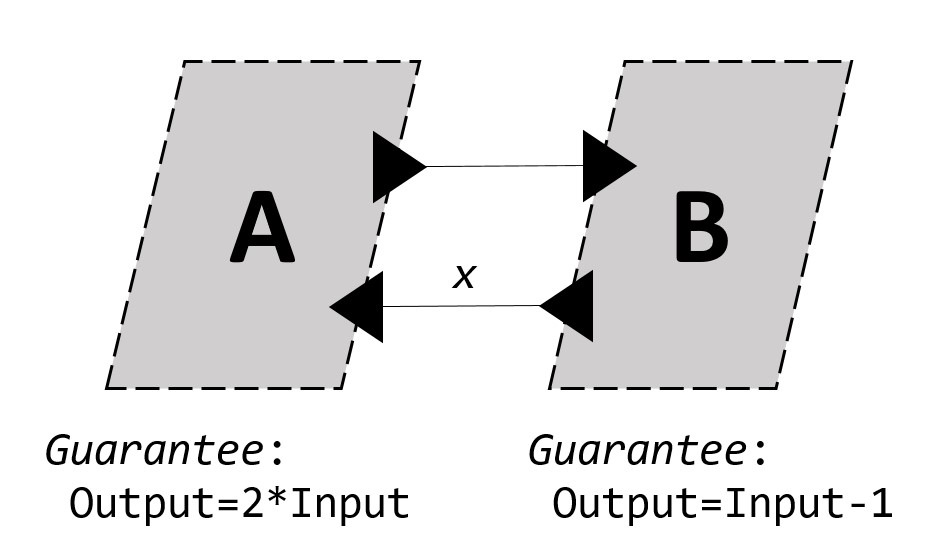
\includegraphics[width=60mm]{motivation.jpg}
\caption{An AADL Model with AGREE Contracts\label{motivation}}
\end{figure}

We use the AADL model annotated with AGREE contracts in Figure \ref{motivation} to illustrate the difference between the original AGREE synchronous semantics and the AADL asynchronous semantics. The model consists of two threads A and B. The AGREE contracts associated with each thread define the input output data relationship. In the AGREE synchronous semantics, the communication between the two threads are instantaneous. And the two contracts have to be satisfied simultaneously. For example, the value of signal \[x = (x_0, x_1, ...)\] is defined by the solution to the fix-point equation x = F(x), where F(x) = 2x -1. That is, \[x_0 = F(x_0), x_1 = F(x_1), x_2 = F(x_2), ...\] This results in x = (1,1,1,…). However, if the two threads are implemented on a single processor, they have to executed in a sequential order, e.g. (A,B,A,B,A,B,…). In AADL a port of a thread represents buffered communication and reading is non-blocking. If the buffer asscoated with a port is empty, a pre-defined constant value or the previous value is used. Given a schedule (A,B,A,B,A,B,…) and an initial value x = 0,  by Kleene iteration: \[x_1 = F(x_0), x_2 = F(x_1), x_3 = F(x_2),...\] This results in x = (0,-1,-3,…). Clearly, the two traces are different. This implies that a property proved with synchronous MoC model may not hold with asynchronous MoC.